
\section{Suche}
\frame{
    \frametitle{Suche}
    \begin{description}
        \item[erneute Suche] Im Suchformular können Sie gegebenenfalls Ihre Suche ändern.
        \item[RSS-Feeds] Alternativ zu den Suchergebnissen können Sie auch Feeds abonnieren.
	Damit können Sie sich schnell über Änderungen in diesen Suchergebnissen informieren
    lassen.
	\item[Trefferliste]
    \end{description}
}

\subsection{Trefferliste}
\frame{
    \frametitle{Suche - Trefferliste}
    Die Suchergebnisse lassen sich noch weiter einschränken:
    \begin{itemize}
        \item nach Artikeltyp
        \item nach Datum
    \end{itemize}
    \begin{figure}[!h]
        \centering
        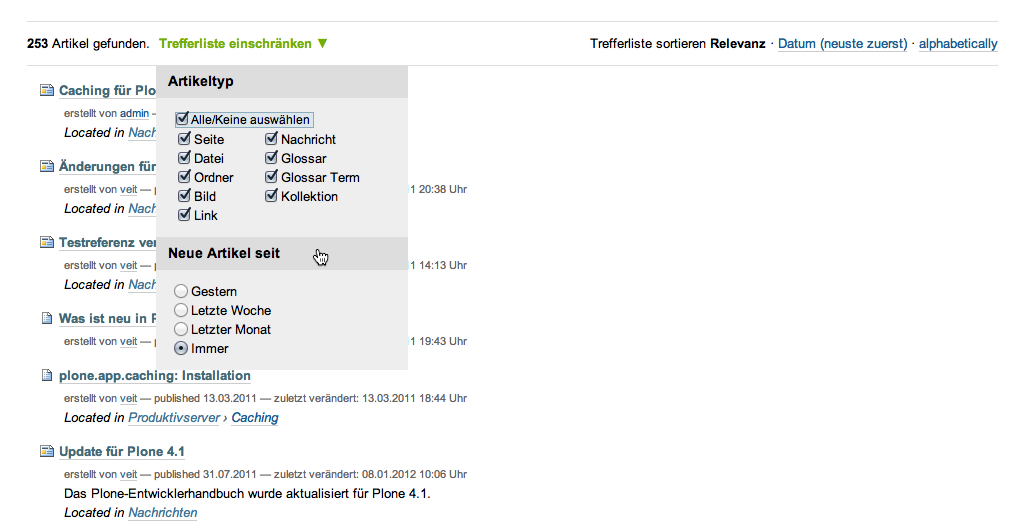
\includegraphics[width=\textwidth]{../res/suchformular.png}
    \end{figure}
}
